\begin{figure*}[t]
\centering
\begin{overpic}[height=1.2in]{Figures/step_1}%
\put(350,-100){(a)}%
\end{overpic}
% 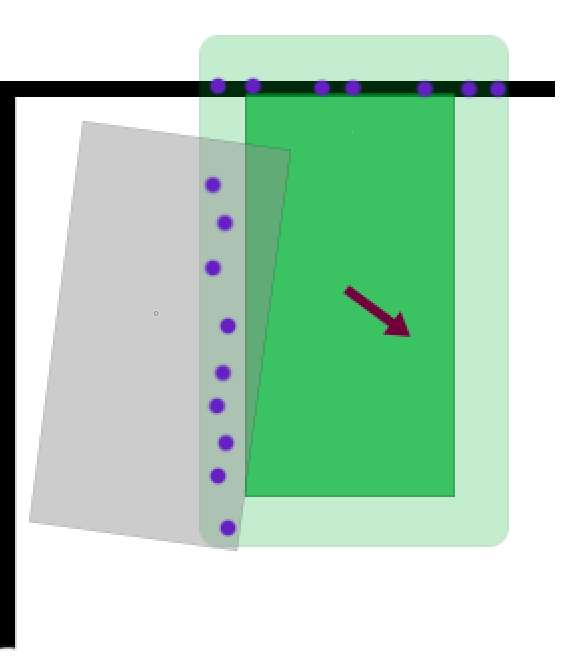
\includegraphics[height=1.2in]{Figures/step_1}
\begin{overpic}[height=1.2in]{Figures/push_3.png}%
\put(350,-100){(b)}%
\end{overpic}
\hspace{0.1in}
% 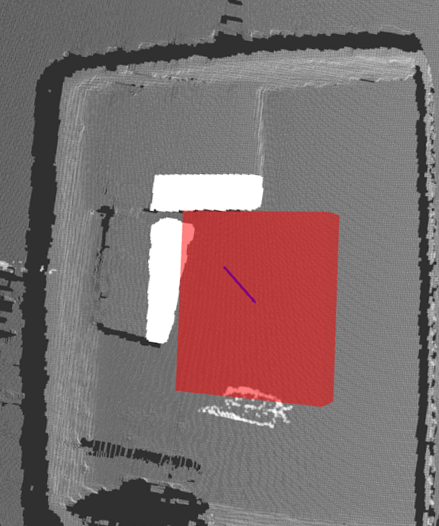
\includegraphics[height=1.2in]{Figures/push_3.png}
\begin{overpic}[height=1.2in]{Figures/tight_push_00.png}%
\put(450,-70){(c)}%
\end{overpic}
% 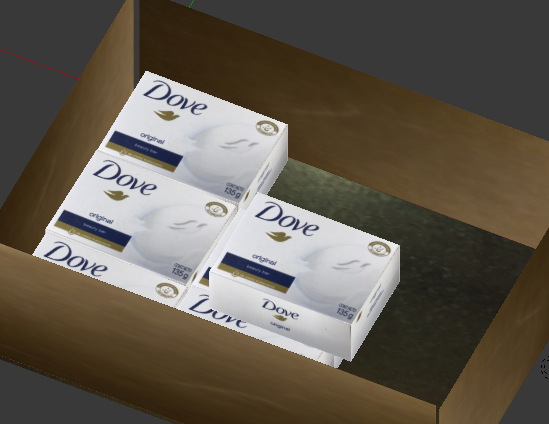
\includegraphics[height=1.2in]{Figures/tight_push_00.png}
\begin{overpic}[height=1.2in]{Figures/tight_push_02.png}%
\put(450,-70){(d)}%
\end{overpic}
% 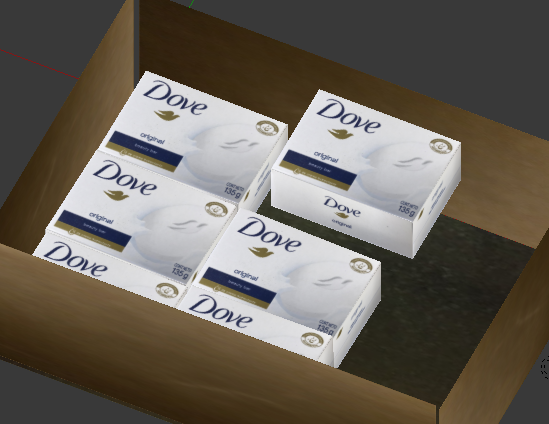
\includegraphics[height=1.2in]{Figures/tight_push_02.png}
\begin{overpic}[height=1.2in]{Figures/tight_push_03.png}%
\put(450,-70){(e)}%
\end{overpic}
% 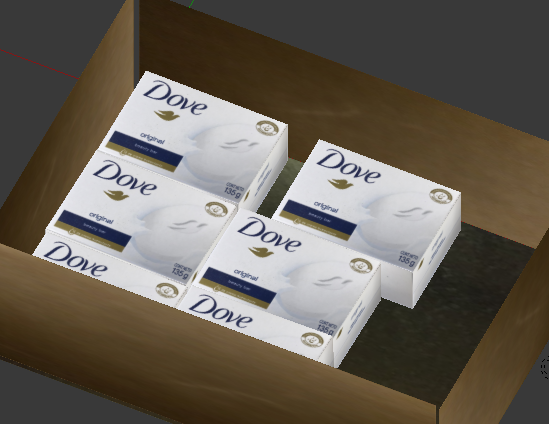
\includegraphics[height=1.2in]{Figures/tight_push_03.png}
% \vspace{-0.1in}
\caption{Adaptive pushing: (a) The black border is the bin and the gray rectangle a previously placed object. The green rectangle represents the target pose for the current object. The light green boundary represents an $\varepsilon$-expanded model that intersects the point cloud at the purple points. These points result in the black vector that pushes the object away from them. (b) A screen shot of a scene's point cloud, where the white points are collision points with previously placed objects and the red volume shows the computed pre-push pose for the new object.
Adaptive pushing in the boundary case (the sixth object). (c)The target object is moving at the upper level and from the pre-push pose to the boundary. (d) The target object is being pushed against the boundary and then pushed down to the bottom level. (e) The target object is moved towards its target pose at the bottom level.
}
\label{fig:adaptive-pushing}
% \vspace{-0.2in}
\end{figure*}



%In the problem of packing in a tight space, failures tend to arise due to the uncertainties from perception of the object and the environment. In order to increase the robustness of packing, we propose a novel manipulation primitive we call "Push-Place". This primitive takes advantage of the compliance of the objects and environments to robustly placing an object in a tight bin. The idea is that instead of directly placing the object to its target position, while still attaching the object to the end-effector, we will first move the object to an intermediate position, then push the object towards its target position. This method has two main benefits: first, in finding the intermediate position, we minimize the probability of collision between the object and the environment;second, during the course of pushing, in addition to moving the target object to its desired position, the interaction between objects will also correct the misalignment of previous packed objects.     

Directly placing objects at the goal pose $\hat{p}^i$ into bin $\btarget$ is prone to placement failures due to errors in perception as well as prior placements. This may result in damaging the objects. A safer alternative is to drop the object from a certain height, right above the goal pose, so as to avoid pressing against previously erroneously placed objects. Still, however, this alternative results in low quality packing. A key realization is that during placement, the object being manipulated will inevitably approach or even collide with other objects or the target container. To sidestep undesirable collisions, an {\em adaptive pushing} primitive is developed, which directly operates over point cloud data for the target bin. 


The process is detailed in algorithm~\ref{algo:PushPlace}. The adaptive pushing begins by growing the object model at the target pose $\hat{p}^i$. Given the uncertainty value $\varepsilon$, the model is enlarged by  $2\varepsilon$ along each dimension. The enlarged model is intersected with the point cloud to retrieve collision points. A collision vector is computed as a vector pointing from a collision point to the center of the object model. Summing all collision vectors yields the displacement vector. By iteratively moving the object model along the unit displacement vector, where the displacement vector is recomputed after each movement, a collision-free pre-push pose for the object is obtained. An example scene is shown in Fig.~\ref{fig:adaptive-pushing}. During the execution, the robot first moves the object above the pre-push pose, then lowers the object to the pre-push pose and finally pushes the object to the target pose. 

% The adaptive pushing primitive begins by moving the picked-up object to a pose with a larger $z$-value than the goal pose $\hat{p}^i$. It then tries to find a set of intermediate target poses for generating collision-free paths for the object and the end-effector as the object is gradually lowered to its final desired pose. The idea behind generating one such intermediate pose is shown in Fig.~\ref{fig:adaptive-pushing}, where a {\em displacement vector} is shown. At any point when a new intermediate pose is to be generated, to counter the potential negative effects caused by pose uncertainty, an $\varepsilon$-expanded model of the object's current estimated pose (i.e., growing the object model by $2\varepsilon$ along each dimension) is intersected with the point cloud. Based on the intersection, a displacement vector defining a new intermediate pose is  generated that guides the object away from potential collisions. 

%An intermediate pose is denoted a {\em pre-push pose}. Algorithm~\ref{algo:PushPlace} outlines the process of finding these pre-push poses. 

\begin{algorithm}
\small
\DontPrintSemicolon
\KwIn{Pointcloud $C$,  target pose $\pose_t$, bounding box size $S$}
\KwOut{Push direction $d$, pre-push pose $\pose_{pre}$  }
$\pose_{pre} \gets \pose_t$ \;
 $bbox \gets$ GenerateBoundingBox($\pose_{pre}, S$)  \;
\While{$bbox$ \normalfont is in collision}{
$C_{collision} \gets$ Intersection($bbox , C$) \;
 $u_{push} \gets$ GeneratePushVector($C_{collision}, \pose_{pre}$)\;
 $\pose_{pre} \gets \pose_{pre} + u_{push}$\;
 \lIf{\normalfont IsLocalMinimum($\pose_{pre}$)}{
    decrease $S$
 }
 $bbox \gets$ GenerateBoundingBox($\pose_{pre}, S$)
}
$d \gets \pose_t - \pose_{pre}$\;
\Return{$d, \pose_{pre}$}\;
\caption{{\sc PushPlace-Planner}}
\label{algo:PushPlace}
\end{algorithm}

\begin{algorithm}
\small
\DontPrintSemicolon
\KwIn{Pointcloud $C$,  target pose $\pose_t$, bounding box size $S$}
\KwOut{Push path $path$ }
$\pose_{higher} \gets \pose_{t}   $\;
$\pose_{higher}.z \gets \pose_{t}.z + obj\_height   $\;
$(d, \pose_{pre}) \gets$ PushPlace-Planner$($C$, \pose_{higher}, S)$  \;
$\pose_{wall} \gets$ ProjectPoseToWall($\pose_{higher})$   \;
$\pose_{down} \gets \pose_{wall}$  \;
$\pose_{down}.z \gets \pose_{wall}.z - obj\_height$   \;
$path \gets (\pose_{wall}, \pose_{pre})$   \;
$path \gets (\pose_{down}, \pose_{wall})$\;
$path   \gets (\pose_{t}, \pose_{down})$    \;
\Return{$path$}\; 
\caption{{\sc TightPushPlace-Planner}}
\label{algo:TightPushPlace}
\end{algorithm}


For special scenario where objects need to be packed tightly with no clearance, in order to place the objects near the boundary robustly, it requires additional steps in pushing. The process is detailed in algorithm~\ref{algo:TightPushPlace}. In this case, since there is no space for pushing in the same layer of the target pose, the target object will first be moved at the upper layer and use the boundary of the container to correct potential noise in the object pose. The compliance of the container boundary will also enable the object to fit the tight gap when the object is pushed down to target level. The process of placing one object to an boundary pose is illustrated in Fig.~\ref{fig:adaptive-pushing}. This procedure is required for each object that is at the boundary of the container. 

% \begin{figure}[t]
% \centering
% 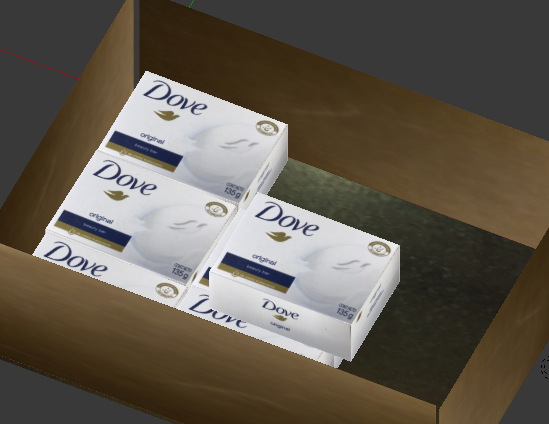
\includegraphics[width=0.15\textwidth]{Figures/tight_push_00.png}
% 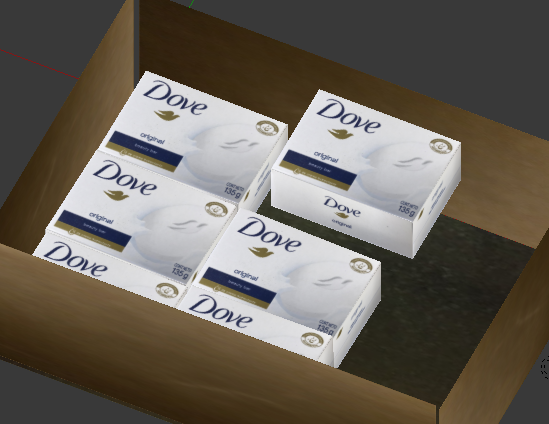
\includegraphics[width=0.15\textwidth]{Figures/tight_push_02.png}
% 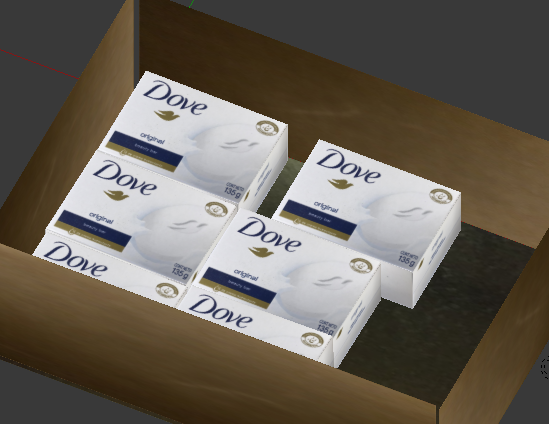
\includegraphics[width=0.15\textwidth]{Figures/tight_push_03.png}
% \vspace{-0.1in}
% \caption{Adaptive pushing in the boundary case (the sixth object). (left)The target object is moving at the upper level and from the pre-push pose to the boundary. (middle) The target object is being pushed against the boundary and then pushed down to the bottom level. (right) The target object is moved towards its target pose at the bottom level.}

% % A screen shot where the green volume is the ground truth pose for the object and the red one is where the object should be moved next.}
% %\label{fig:workspace}
% \label{fig:tight-pushing}
% \vspace{0.1in}
% \end{figure}

%Line 1-2 initialize the pre-push pose $\pose_{pre}$ and the bounding box $bbox$ generated at $\pose_{pre}$. The function GenerateBoundingBox generates a bounding box centered at the given pose with the given size. In line 2, the size $S$ is bigger than the actual size of the object to reflect the uncertainties of the estimated pose. Line 3-8 of the algorithm iteratively tries to find a collision-free pre-push pose. The strategy is to move the bounding box towards the direction that will decrease the collision region. In line 4, Function Intersection($bbox, C$) will calculate the intersection points between bounding box $bbox$ and the environment pointcloud $C$. $C_{collision}$ will be passed to function GeneratePushVector to generate a local unit vector to move the current pre-push pose. In function GeneratePushVector($C_{collision}, \pose_{pre}$), all the vectors from points of $C_{collision}$ to the pre-push pose $\pose_{pre}$ are normalized, the summation of all these unit vectors is returned as the local push vector $u_{push}$. Then $u_{push}$ is used to update the pre-push pose $\pose_{pre}$. At narrow region, this local optimization process can be stuck at local minimum. The strategy we used is to reduce the size $S$ for generating bounding box. In the experiments, this usually helped to find a valid pre-push pose.

